%%%%%%%%%%%%%%%%%%%%%%%%%%%%%%%%%%%%%%%%%%%%%%%%%%%%%%%%%%%%%%%%%
\documentclass[12pt, a4paper, notitlepage, onecolumn]{article}
\usepackage[UKenglish]{babel}                   % UK style
\usepackage[utf8]{inputenc}
\usepackage[margin=1in]{geometry}               % Margin size
\usepackage{hyperref}                           % Coloured hyperlinks
  \hypersetup{colorlinks = true}
\usepackage{lmodern}                            % Modern fonts
\usepackage{graphicx}                           % For figures
\usepackage[percent]{overpic}                   % For figures with text overlay
\usepackage{amsmath,amssymb}                    % Mathematical symbols
\usepackage{mathtools}
\usepackage{siunitx}                            % SI-units
%\sisetup{exponent-product = \cdot}             % Dot product instead of cross product
\sisetup{separate-uncertainty = true}           % Plus-minus uncertainty
\usepackage{physics}                            % Elegant equations in physics
\usepackage{booktabs}                           % Nice lines, for instance in tables
\usepackage[font=small,labelfont=bf]{caption}% Caption
\usepackage{float}                              % Table do not move with [H].
\usepackage{subcaption}                         % For subfigures
\usepackage[en-GB]{datetime2}                   % UK date format
\usepackage{listings}                           %Source code
\usepackage{feynmp}                             % Feynman diagrams
\DeclareGraphicsRule{*}{mps}{*}{}               % Include Feynman diagrams
\usepackage{scalerel}
\newcommand{\mylbrace}[2]{\vspace{#2pt}\hspace{6pt}\scaleleftright[\dimexpr5pt+#1\dimexpr0.06pt]{\lbrace}{\rule[\dimexpr2pt-#1\dimexpr0.5pt]{-4pt}{#1pt}}{.}}
\newcommand{\myrbrace}[2]{\vspace{#2pt}\scaleleftright[\dimexpr5pt+#1\dimexpr0.06pt]{.}{\rule[\dimexpr2pt-#1\dimexpr0.5pt]{-4pt}{#1pt}}{\rbrace}\hspace{6pt}}
\usepackage{xspace}                             % Fancy LHCb symbols
\usepackage{upgreek}
\def\pythia{\mbox{\textsc{Pythia}}\xspace}
\def\evtgen{\mbox{\textsc{EvtGen}}\xspace}
\def\photos{\mbox{\textsc{Photos}}\xspace}

%%%%%%%%%%%%%%%%%%%%%%%%%%%%%%%%%%%%%%%%%%%%%%%%%%%%%%%%%%%%%%%
\title{Determination of the CKM angle $\gamma$ in $B^\pm\to DK^\pm, D\pi^\pm$ decays and strong phase determination of $D\to K^+K^-\pi^+\pi^-$ at BESIII}
\author{Martin Duy Tat}
\date{\today}
\numberwithin{equation}{section}
%%%%%%%%%%%%%%%%%%%%%%%%%%%%%%%%%%%%%%%%%%%%%%%%%%%%%%%%%%%%%%%
\begin{document}
\maketitle
\begin{abstract}
\noindent Write abstract at the end
\end{abstract}
%%%%%%%%%%%%%%%%%%%%%%%%%%%%%%%%%%%%%%%%%%%%%%%%%%%%%%%%%%%%%%%
\section{Introduction}
\noindent In the Standard Model, CP-violation can occur if the CKM matrix has a non-trivial weak phase. This is studied by measuring the lengths and angles of the Unitary Triangle of the CKM matrix. In particular, the angle $\gamma = \arg(-V_{ud}V^*{ub}/V_{cd}V^*{cb})$ is the only angle that can be measured at tree level, with negligible theoretical uncertainties. A precise determination of $\gamma$ is therefore a good Standard Model benchmark which can be compared with indirect determinations from other CKM observables that are sensitive to new physics.

Sensitivity to $\gamma$ can be achieved through interference between the $b\to c\bar{u}s$ and $b\to u\bar{c}s$ transitions. A powerful decay mode is $B^\pm\to DK^\pm$, where $D$, a superposition of $D^0$ and $\bar{D^0}$, subsequently decays to a self-conjugate state. This is illustrated in Fig. \ref{fig_feynman_B2DK}. On the left, the colour favoured decay $B^-\to D^0K^-$ is shown, while on the right is the decay colour suppressed $B^-\to\bar{D^0}K^-$. Interference is observed when $D^0$ and $\bar{D^0}$ decays to a common final state.

\begin{figure}[H]
  \centering
  \vspace{0.3cm}
  \begin{subfigure}{0.5\textwidth}
    \centering
    \begin{fmffile}{fgraph/fgraph_BtoDK1}
      \setlength{\unitlength}{0.4cm}
      \begin{fmfgraph*}(9,6)
        \fmfstraight
        \fmfleft{i1,B,i2,t1,t2,t3,t9,t10}
        \fmfright{o1,D,o2,t4,t5,o3,K,o4}
        \fmflabel{$\bar{u}$}{i1}
        \fmflabel{$b$}{i2}
        \fmfv{l.d=20,l.a=180,l={$B^-$\mylbrace{30}{-8}}}{B}
        \fmflabel{$\bar{u}$}{o1}
        \fmflabel{$c$}{o2}
        \fmflabel{$\bar{u}$}{o3}
        \fmflabel{$s$}{o4}
        \fmfv{l.d=15,l.a=0,l={\myrbrace{30}{-12}}$D^0$}{D}
        \fmfv{l.d=15,l.a=0,l={\myrbrace{30}{11}}$K^-$}{K}
        \fmf{fermion}{o1,i1}
        \fmf{fermion,tension=1.5}{i2,v1}
        \fmf{fermion}{v1,o2}
        \fmf{phantom,tension=1.5}{t9,v2}
        \fmf{boson,label=$W$,label.side=left,tension=0}{v1,v2}
        \fmf{fermion}{v2,o4}
        \fmf{fermion}{o3,v2}
      \end{fmfgraph*}
    \end{fmffile}
    \vspace{0.5cm}
    \caption{$B^-\to D^0K^-$}
  \end{subfigure}%
  \begin{subfigure}{0.5\textwidth}
    \centering
    \begin{fmffile}{fgraph/fgraph_BtoDK2}
      \setlength{\unitlength}{0.4cm}
      \begin{fmfgraph*}(9,6)
        \fmfstraight
        \fmfleft{i1,t1,t2,B,t9,t10,i2}
        \fmfright{o1,K,o2,t4,t5,o3,D,o4}
        \fmflabel{$\bar{u}$}{i1}
        \fmflabel{$b$}{i2}
        \fmfv{l.d=20,l.a=180,l={$B^-$\mylbrace{100}{-8}}}{B}
        \fmflabel{$\bar{u}$}{o1}
        \fmflabel{$s$}{o2}
        \fmflabel{$\bar{c}$}{o3}
        \fmflabel{$u$}{o4}
        \fmfv{l.d=15,l.a=0,l={\myrbrace{30}{13}}$\bar{D^0}$}{D}
        \fmfv{l.d=15,l.a=0,l={\myrbrace{30}{-13}}$K^-$}{K}
        \fmf{fermion}{o1,i1}
        \fmf{fermion,tension=1.5}{i2,v1}
        \fmf{fermion}{v1,o4}
        \fmf{phantom,tension=1.5}{t2,v2}
        \fmf{boson,label=$W$,label.side=left,tension=0}{v1,v2}
        \fmf{fermion}{v2,o2}
        \fmf{fermion}{o3,v2}
      \end{fmfgraph*}
    \end{fmffile}
    \vspace{0.5cm}
    \caption{$B^-\to\bar{D^0}K^-$}
  \end{subfigure}
  \caption{Feynman diagrams of $B^-\to DK^-$ decays}
  \label{fig_feynman_B2DK}
\end{figure}

A wide range of subsequent $D$ decays has been studied. Most recently, the measurement $\gamma = (68.7^{+5.2}_{-5.1})^\circ$ from an analysis of the decay modes $D\to K_S^0\pi^+\pi^-$ and $D\to K_S^0K^+K^-$ was obtained, which is the single most precise measurement of $\gamma$. In this project, the decay $B^\pm\to DK^\pm$, where $D\to K^+K^-\pi^+\pi^-$, is considered. An initial study showed that a precision of $\SI{14}{\degree}$ is achievable with a sample of $1000$ $B^\pm\to DK^\pm$ candidates. From similar decay channels, it is estimated that $2000$ candidates can be reconstructed from the combined Run $1$+$2$ LHCb dataset.

A significant challenge with this analysis is that the $D\to K^+K^-\pi^+\pi^-$ decay is a multi-body decay, so the strong phase difference between the $D^0$ and $\bar{D^0}$ decays varies non-trivially across phase space. Moreover, with four particles in the final state phase space becomes five-dimensional. To predict this strong phase difference, a decay model, such as one developed by LHCb, may be used. However, such a model introduces systematic uncertainties due to modelling.

In this analysis, a model-independent approach is chosen, in which strong phases are determined at a charm factory, BESIII, where, quantum correlated $D^0\bar{D^0}$ pairs are produced at the $\psi(3770)$ resonance. The amplitude-averaged strong phases are measured in bins of the $D\to K^+K^-\pi^+\pi^-$ phase space. The choice of binning scheme may enhace the sensitivity to $\gamma$. However, a poor choice of binning scheme may only decrease the statistical sensitivity, but not bias the result. With a model-independent approach, one therefore eliminates the systematic uncertainty due to modelling.

%%%%%%%%%%%%%%%%%%%%%%%%%%%%%%%%%%%%%%%%%%%%%%%%%%%%%%%%%%%%%%%
\section{Formalism}
\subsection{\texorpdfstring{$\gamma$}{gamma} sensitity through \texorpdfstring{$B^\pm$}{B} decays}
The amplitude of $B^\pm\to DK^\pm$ is a coherent sum of the diagrams in Fig. \ref{fig_feynman_B2DK},

\begin{align}
  \mathcal{A}(B^-\to DK^-) =& \mathcal{A}_D + r_B^{DK}e^{i(\delta_B^{DK} - \gamma)}\mathcal{A}_{\bar{D}}, \label{eq_Bm2DKm} \\
  \mathcal{A}(B^+\to DK^+) =& \mathcal{A}_{\bar{D}} + r_B^{DK}e^{i(\delta_B^{DK} + \gamma)}\mathcal{A}_D, \label{eq_Bp2DKp}
\end{align}
where $r_B$ is the relative magnitude of the diagrams in Fig. \ref{fig_feynman_B2DK} and $A_{D, \bar{D}}$ are the amplitudes for the $D$ decay as a function of phase space. $\delta_B^{DK}$ is the strong phase of the $B^\pm\to DK^\pm$ decay and is invariant under CP, while $\gamma$ is the weak phase that swaps sign under CP.

The $B^\pm\to DK^\pm$ decay rate is considered in $2\times N$ bins of phase space, labelled $i = -N, ..., N$, excluding zero. Bin $i$ is related to $-i$ by a CP transformation. When integrating the square of Eqs. \eqref{eq_Bm2DKm}-\eqref{eq_Bp2DKp}, the $B^-\to DK^-$ decay rate in bin $i$ and $B^+\to DK^+$ decay rate in bin $-i$ are

\begin{align}
  \Gamma^-_i = h_{B^-}\Big[F_i + \big((x_-^{DK})^2 + (y_-^{DK})^2\big)F_{-i} + 2\sqrt{F_iF_{-i}}\big(x_-^{DK}c_i + y_-^{DK}s_i\big)\Big], \label{eq_Bm2DKm_rate} \\
  \Gamma^+_{-i} = h_{B^+}\Big[F_i + \big((x_+^{DK})^2 + (y_+^{DK})^2\big)F_{-i} + 2\sqrt{F_iF_{-i}}\big(x_+^{DK}c_i + y_+^{DK}s_i\big)\Big], \label{eq_Bp2DKp_rate}
\end{align}
where

\begin{equation}
  c_i = \frac{\int_i\dd{\vb{x}}\abs{\mathcal{A}_D}\abs{\mathcal{A}_{\bar{D}}}\cos(\Delta\delta_D)}{\sqrt{\int_i\dd{\vb{x}}\abs{\mathcal{A}_D}^2\int_i\dd{\vb{x}}\abs{\mathcal{A}_{\bar{D}}}^2}}, \quad s_i = \frac{\int_i\dd{\vb{x}}\abs{\mathcal{A}_D}\abs{\mathcal{A}_{\bar{D}}}\sin(\Delta\delta_D)}{\sqrt{\int_i\dd{\vb{x}}\abs{\mathcal{A}_D}^2\int_i\dd{\vb{x}}\abs{\mathcal{A}_{\bar{D}}}^2}}, \quad F_i = \frac{\int_i\dd{\vb{x}}\abs{\mathcal{A}_D}^2}{\sum_i\int_i\dd{\vb{x}}\abs{\mathcal{A}_D}^2}.
  \label{eq_hadronic_parameters}
\end{equation}
$c_i$ and $s_i$ is the strong phase difference $\Delta\delta_D$ between the $B^-\to D^0K^-$ and $B^+\to\bar{D^0}K^+$ decays, amplitude-averaged over bin $i$. $F_i$ is the fractional yield of $B^-\to D^0K^-$ in bin $i$, and assuming CP conservation in $D$ decays the corresponding fractional yield of $B^+\to D^0K^+$ in bin $i$ is $F_{-i}$. $h_{B^\pm}$ are a normalization constants.

Furthermore, we define the CP observables

\begin{equation}
  x_\pm^{DK} = r_B^{DK}\cos(\delta_B^{DK}\pm\gamma), \quad  y_\pm^{DK} = r_B^{DK}\sin(\delta_B^{DK}\pm\gamma).
  \label{eq_xy_cp}
\end{equation}

Therefore, by counting the number of $B^\pm\to DK^\pm$ decays in bins of phase space, one can do a simultaneous fit of Eqs. \eqref{eq_Bm2DKm_rate}-\eqref{eq_Bp2DKp_rate} one can obtain the CP observables $x_\pm^{DK}$ and $y_\pm^{DK}$. It is the interference terms in Eqs. \eqref{eq_Bm2DKm_rate}-\eqref{eq_Bp2DKp_rate} which causes CP-violation. A clever choice of binning scheme will enhance these interferences, which makes the fit more sensitive to the CP-observables, which can then be interpreted in terms of $\gamma$, $\delta_B^{DK}$ and $r_B^{DK}$.

The fit will require external inputs for $c_i$ and $s_i$ from BESIII. In addition, the $F_i$ may either be obtained from flavour tagged $D$ decays, or treated as floating variables in the fit. In this analysis, the second method is preferred in order to reduce systmatic uncertainties due to differences in phase space efficiencies. However, to constrain the $F_i$ and improve the fit stability, the analogous decay mode $B^\pm\to D\pi^\pm$, which has a similar selection and detector signature, is also included as a signal mode in the simultaneous fit. The common topology also means the $F_i$ will be the same, but this mode has a much smaller CP-violation due to interference because $r_B^{D\pi}$ is expected to be much smaller than $r_B^{DK}$.

Since not all CP variables are independent, the fit stability is improved by introducing the variables

\begin{equation}
  x_\xi^{D\pi} = \Re(\xi^{D\pi}), \quad y_\xi^{D\pi} = \Im(\xi^{D\pi}), \quad \xi^{D\pi} = \frac{r_B^{D\pi}}{r_B^{DK}}e^{i(\delta_B^{D\pi} - \delta_B^{DK})}.
\end{equation}

Therefore, in the final fit the CP observables are $x_\pm^{DK}$, $y_\pm^{DK}$, $x_\xi^{D\pi}$ and $y_\xi^{D\pi}$.

\subsection{Strong phase and quantum correlations}
The strong phase differences $\Delta\delta_D$ of $D\to K^+K^-\pi^+\pi^-$ decays are directly measured in quantum correlated $D^0\bar{D^0}$ decays, using the method of double tagging. This method involves reconstructing either one or both $D$ meson decays. If one of the $D$ mesons is reconstructed in some mode final state $f$, one can obtain the single tag yield of $f$. If both $D$ decays are reconstructed in final states $f$ and $g$, the corresponding double tag yield is obtained. The double tag method is useful when one of the $D$ mesons is reconstructed as $D\to K^+K^-\pi^+\pi^-$, known as the signal mode, and the other $D$ meson decays to a known tag mode.

In particular, if the tag mode is a flavour tag, such as $K^-\pi^+$, one can deduce, through quantum correlations, the original flavour of the $D$ meson on the signal side. One can therefore define a quantity $K_i$, which is yield of flavour tagged $D^0\to K^+K^-\pi^+\pi^-$ events in bin $i$. The corresponding yield for $\bar{D^0}$ decays are then placed in bin $-i$.

The sensitivity to the cosine of the strong phase occurs when the tag mode is a CP eigenstate, or some self-conjugate state with known CP-even fraction $F_+$. The yield of CP tagged $D\to K^+K^-\pi^+\pi^-$ events in bin $i$ is given by

\begin{equation}
  M_i^\pm = \frac{S_\pm}{2S_f}\Big[K_i - 2c_i(2F_+ - 1)\sqrt{K_iK_{-i}} + K_{-i}\Big],
  \label{eq_Mi}
\end{equation}
where $S\pm$ and $S_f$ are the single tag yields of the CP and flavour tag modes used, respectively. For CP even (odd) modes, $F_+ = +1$ ($-1$). To get sensitivity to the sine of the strong phase, the tag mode must be a self-conjugate mode, and the analogous expression is

\begin{equation}
  M_{ij} = \frac{N_{D\bar{D}}}{2S_fS_f'}\Big[K_iK'_{-j} + 2\sqrt{K_iK'_{-j}K_{-i}K'_j}(c_i'c_j + s_i's_j) + K_{-i}K'_j\Big],
  \label{eq_Mij}
\end{equation}
where $N_{D\bar{D}}$ is the total number of $D^0\bar{D^0}$ pairs produced. Here both final states $f$ and $f'$ are reconstructed in bins $(i, j)$ of phase space. In the simplest case, $f = f' = K^+K^-\pi^+\pi^-$, in which $c'_i = c_i$ and $s'_i = s_i$ are all obtained from a fit. One can also choose $f = K^+K^-\pi^+\pi^-$ and $f' = K_S\pi^+\pi^-$, for which the strong phases are already well known.

Once all single and double tag yields have been extracted, a maximum likelihood fit is performed to obtain $c_i$ and $s_i$. A table of all tag modes is shown in Table \ref{table_tag_modes}.

\begin{table}[H]
  \centering
  \caption{Tag modes used in the BESIII double tag analysis. Subsequent decays are shown in parentheses. CP conjugates of flavour modes are implied.}
  \label{table_tag_modes}
  \begin{tabular}{cccc} 
    \toprule
    Flavour & CP even & CP odd & Self conjugate \\
    \midrule
    $K^-\pi^+$, $K^-\pi^+\pi^0$, & $K^+K^-$, $\pi^+\pi^-$,                  & $K_S^0\pi^0$, $K_S^0\phi$,                  & $K_S^0\pi^+\pi^-$, \\
    $K^-\pi^+\pi^-\pi^+$,        & $\pi^+\pi^-\pi^0$, $K_S^0\pi^0\pi^0$,    & $K_S^0\eta(\gamma\gamma, \pi^+\pi^-\pi^0)$, & $K^+K^-\pi^+\pi^-$ \\
    $K^- e^+\nu_e$               & $K_L^0\pi^0$, $K_L^0\eta(\gamma\gamma)$, & $K_S^0\omega(\pi^+\pi^-\pi^0)$,             & \\
                                 & $K_L^0\omega(\pi^+\pi^-\pi^0)$           & $K_S^0\eta'(\pi^+\pi^-\eta(\gamma\gamma), \pi^+\pi^-\gamma)$  & \\
    \bottomrule
  \end{tabular}
\end{table}

Currently, BESII has collected $\SI{2.932}{\femto\per\barn}$ of data at the $\psi(3770)$ resonance during $2010$-$2011$, which is unsufficient for doing a maximum likelihood fit. However, a significant increase in data is expected from $2022$, allowing for a precise determination of $c_i$ and $s_i$.
%%%%%%%%%%%%%%%%%%%%%%%%%%%%%%%%%%%%%%%%%%%%%%%%%%%%%%%%%%%%%%%
\section{LHCb detector}
\noindent The LHCb is a single arm forward spectrometer designed to study beauty and charm hadrons in $pp$ collisions at the LHC. The main components important for this analysis are the high precision tracking system and the two Ring Imaging Cherencov counters (RICH1 and RICH2).

The tracking system includes the Vertex Locator (VELO). The VELO consists of silicon strip modules close to the interaction point, which provides high precision tracking and identification of displaced secondary vertices that are important for beauty and charm physics. A dipole magnet with bending power of about $\SI{4}{\tesla\meter}$ together with three tracking stations of silicon strip detectors and straw drift tubes placed downstream provides a measurement of the momentum of charged particles with an uncertainty of $0.5\%$ at low momentum at $1.0\%$ at $\SI{200}{\giga\eV}$. The impact parameter is measured with a resolution of $(15 + 29/p_T)\si{\micro\meter}$, where $p_T$ is the transverse momentum.

The two RICH detectors, together with the tracking system and the calorimeter system, separates kaons from pions. The upstream RICH1 detector covers the lower momentum range up to $\SI{60}{\giga\eV}$ while the downstream RICH2 covers the higher momentum range from $\SI{15}{\giga\eV}$ to $\SI{100}{\giga\eV}$.

To model the kinematic distributions of signal and background components and determine selection efficiencies, simulations of $pp$ collisions are generated in \pythia. Decays are described by \evtgen and final state radiation is generated witih \photos. In addition, models of decay amplitudes are incorporated using the AmpGen framework.

%%%%%%%%%%%%%%%%%%%%%%%%%%%%%%%%%%%%%%%%%%%%%%%%%%%%%%%%%%%%%%%
\section{Binning scheme}
\label{section_binning_scheme}
\noindent In a three-body decay, such as $D\to K_S^0\pi^+\pi^-$, the two-dimensional phase space may be visualized in a two-dimensional Dalitz plot. In an analysis analogous to $D\to K^+K^-\pi^+\pi^-$, the Dalitz space was separated into bins of similar strong phase, such that the amplitude-averaged strong phases $c_i$ and $s_i$ were not diluted due to binning. In addition, the Dalitz plot was split symmetrically into bins with positively and negatively indexed bins, such that most Cabbibo favoured resonances and doubly suppressed Cabbibo resonances were on opposite sides of each other. Such a clever choice of bins will therefore enhance the interference terms in Eqs. \eqref{eq_Bm2DKm_rate}-\eqref{eq_Bp2DKp_rate}, and thus enhance the sensitivity to CP-violation effects.

A similar choice of binning must be determined for the four-body decay mode $D\to K^+K^-\pi^+\pi^-$. While similar in many ways, this phase space is five-dimensional and cannot easily be visualized. Instead, an amplitude model is used to predict the decay amplitude and strong phase difference. The model, implemented using the AmpGen framework, takes in the momenta of the $D$ daughter particles, and the output is used to calculate the $D\to K^+K^-\pi^+\pi^-$ decay amplitude $\mathcal{A}(D)$. One can then define

\begin{equation}
  \frac{\mathcal{A}(D^0)}{\mathcal{A}(\bar{D^0})}\equiv r_De^{i\Delta\delta_D},
\end{equation}
where $\Delta\delta_D$ is the strong phase difference and $r_D$ is the relative magnitude, both of which vary across phase space. A convenient binning scheme would therefore be equal $\Delta\delta_D$ separation in each bin such that areas of phase space with similar strong phases are grouped together in the same bins.

Under a CP transformation, $\Delta\delta_D\to -\Delta\delta_D$ and $\ln(r_D)\to -\ln(r_D)$. For $\ln(r_D) > 0$, the $\bar{D^0}\to K^+K^-\pi^+\pi^-$ decay is suppressed, relative to $D^0\to K^+K^-\pi^+\pi^-$, while the converse is true for $\ln(r_D) < 0$. The interference terms in Eqs. \eqref{eq_Bm2DKm_rate}-\eqref{eq_Bp2DKp_rate} may therefore be enhanced if the positively and negatively indexed bins are split along the line $\ln(r_D) = 0$.

A measure of the binning scheme sensitivity to CP observables is taking the ratio of the statistical sensitivity to $x_\pm$ and $y_\pm$ in a binned fit and the corresponding statistical sensitivity with infinitely many bins. It can be shown that

\begin{equation}
  Q^2 = \frac{1}{2}\big(Q^2_+ + Q^2_-\big), \quad Q^2_\pm = 1 - \sum_i\frac{F_iF_{-i}\big(1 - c_i^2 - s_i^2\big)}{N_i^\pm},
  \label{eq_binning_Q}
\end{equation}
where $N_i^\pm$ are calculated using Eqs. \eqref{eq_Bm2DKm_rate}-\eqref{eq_Bp2DKp_rate}. To maximize $Q$, the bin boundaries along $\Delta\delta_D$ are moved symmetrically around $\Delta\delta_D = 0$.

To assess the binning scheme performance, $1000$ toy experiments with $2000$ $B^\pm$ candidates was generated with the amplitude model using AmpGen. The input parameters used were $\gamma = \SI{75}{degree}$, $\Delta_B = \SI{130}{\degree}$ and $r_B = 0.1$. An unbinned maximum likelihood fit was performed in order to establish a benchmark for the $\gamma$ precision obtainable. It was found that the average precision to $\gamma$ was $\Delta\gamma = \SI{11}{\degree}$.

For the particular choice of $2\times 8$ bins, the optimal binning scheme is shown in Fig. \ref{fig_binning_scheme}. Eq. \eqref{eq_binning_Q} gives $Q = 0.90$, which indicates that $10\%$ sensitivity is lost due to binning. A binned maximum likelihood fit was performed using the binning scheme in Fig. \ref{fig_binning_scheme} and Eqs. \eqref{eq_Bm2DKm_rate}-\eqref{eq_Bp2DKp_rate} to extract $x_\pm^{DK}$ and $y_\pm^{DK}$. The parameters $c_i$, $s_i$ and $F_i$ were calculated using Monte Carlo integration of Eqs. \eqref{eq_hadronic_parameters} with $\mathcal{A}(D)$ calculated using the amplitude model. Finally, $\gamma$, $\delta_B$ and $r_B$ where obtained by fitting $x_\pm^{DK}$ and $y_\pm^{DK}$ using Eqs. \eqref{eq_xy_cp}.

The mean and standard deviation of the pull distributions of $x_\pm^{DK}$, $y_\pm^{DK}$, $\gamma$, $\delta_B$ and $r_B$ are shown in Table \ref{table_pull_study}. All pulls are consistent with zero mean and unit standard deviation, with the exception of $r_B$, which has a bias. Similar behaviour has been found in similar analyses.

\begin{figure}[H] 
  \centering
  \begin{subfigure}{0.5\textwidth}
    \centering
    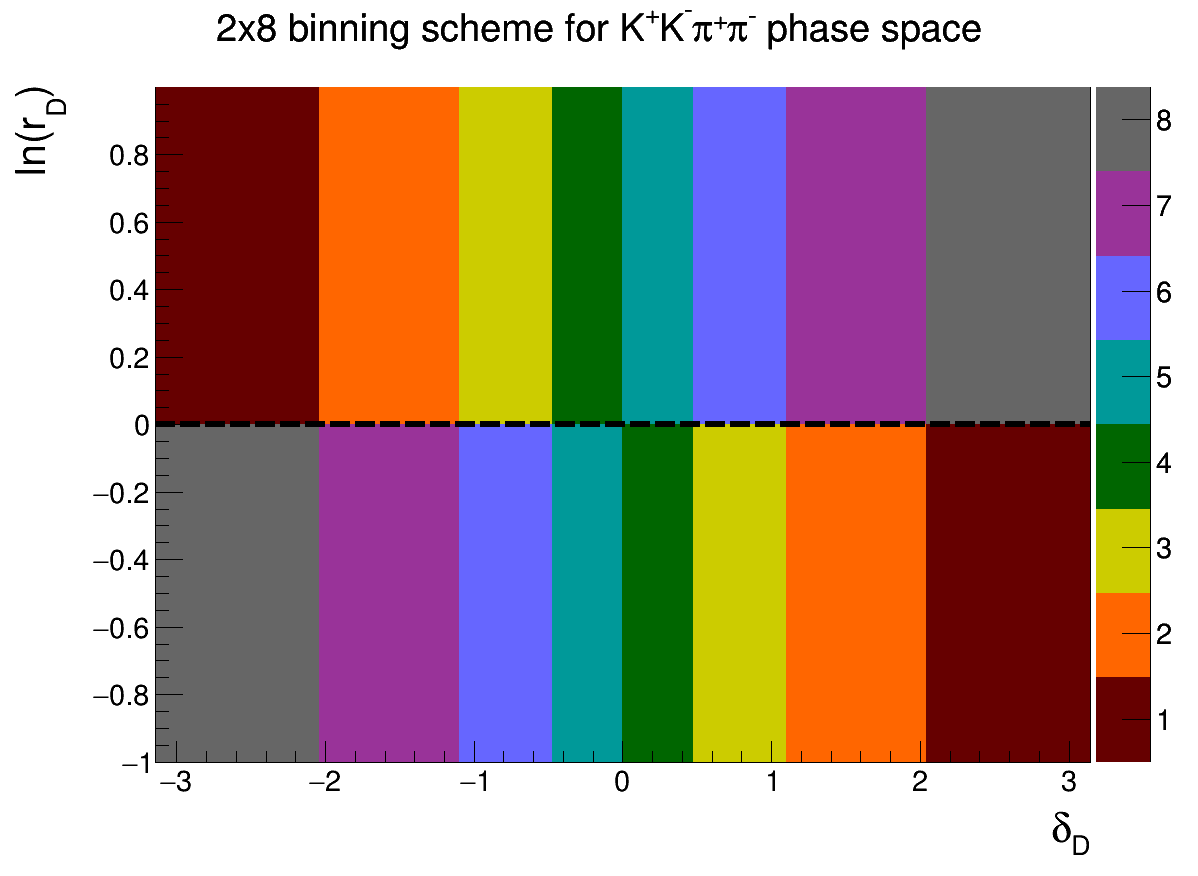
\includegraphics[width=1\textwidth]{Plots/BinningSchemePlot.png}
    \caption{Binning scheme definition for $2\times 8$ bins}
    \label{fig_binning_scheme}
  \end{subfigure}%
  \begin{subfigure}{0.5\textwidth}
    \centering
    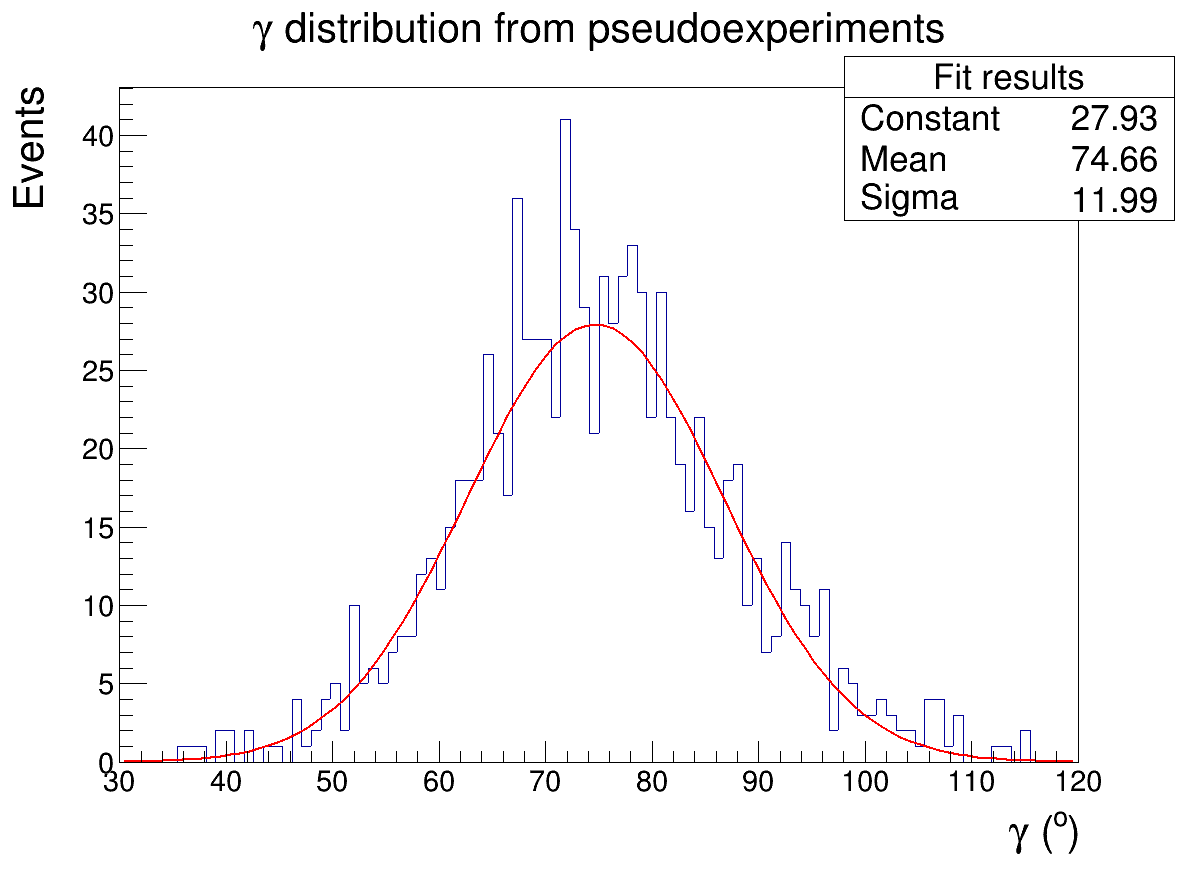
\includegraphics[width=1\textwidth]{Plots/GammaDistribution8BinsVariableWidth.png}
    \caption{Distribution of $\gamma$ from toy study}
    \label{fig_gamma_pull_study}
  \end{subfigure}
  \caption{}
\end{figure}

The fitted values of $\gamma$ from all the toy experiments are shown in Fig. \ref{fig_gamma_pull_study}. It was found that the precision achievable with binned fit, with the optimized $2\times 8$ binning scheme, was $\SI{12.0(4)}{\degree}$. This is consistent with the binning $Q$ value and the unbinned fit benchmark.

\begin{table}[H]
  \centering
  \caption{The pull distribution mean and standard deviation from toy study.}
  \label{table_pull_study}
  \begin{tabular}{ccc} 
    \toprule
    Observable & Mean                 & Standard deviation \\
    \toprule
    $x_+^{DK}$ & $\SI{3.7(33)e-2}{}$  & $\SI{9.80(26)e-1}{}$ \\
    $x_-^{DK}$ & $\SI{1.4(33)e-2}{}$  & $\SI{9.48(26)e-1}{}$ \\
    $y_+^{DK}$ & $\SI{2.6(34)e-2}{}$  & $\SI{10.04(28)e-1}{}$ \\
    $y_-^{DK}$ & $\SI{-1.7(31)e-2}{}$ & $\SI{9.24(26)e-1}{}$ \\
    $\gamma$   & $\SI{4.9(33)e-2}{}$ & $\SI{9.77(29)e-1}{}$ \\
    $\delta_B$ & $\SI{4.9(33)e-2}{}$ & $\SI{9.86(26)e-1}{}$ \\
    $r_B$      & $\SI{1.72(32)e-1}{}$ & $\SI{9.46(26)e-1}{}$ \\
    \bottomrule
  \end{tabular}
\end{table}

%%%%%%%%%%%%%%%%%%%%%%%%%%%%%%%%%%%%%%%%%%%%%%%%%%%%%%%%%%%%%%%
\section{\texorpdfstring{$B^\pm$}{B} candidate selection}
\subsection{Signal candidate requirements}
\noindent The $B^\pm\to Dh^\pm$ candidates, with $h^\pm = \pi^\pm, K^\pm$ and $D^\to K^+K^-\pi^+\pi^-$, are reconstructed from five charged tracks. The standard track and trigger requirements mainly follows that of Ref. \ref{}. To ensure that there is a real $D$ meson in the selection, the four charged tracks from $D$ are required to be inside a mass window of $\SI{25}{\mega\eV}$ of the PDG mass. Then the tracks are refitted with their invariant mass constrained to the PDG value and its momentum is required to point back to the primary vertex. A cut on the $\chi^2$ at $\ln(\chi^2) < 3$ will remove most of the sideband background in the $D$ invariant mass.

A mutually exclusive Particle Identification (PID) cut is imposed to separate the $B^\pm\to D\pi^\pm$ and $B^\pm\to DK^\pm$ candidates. In addition the $K^\pm$ daughter from $D$ and the direct $h^\pm$ daughter from $B^\pm$ are required to have momentum $p < \SI{100}{\giga\eV}$ to be inside the optimal range for the RICH to distinuish pions and kaons.

More specialized selection, discussed in Sections \ref{subsection_BDT}-\ref{subsection_charmless}, are considered to remove specific backgrounds.

\subsection{Boosted Decision Tree}
\label{subsection_BDT}
\noindent Combinatorial backgrounds form the largest part of the background after the standard selection is performed. A Boosted Decision Tree (BDT) was used to remove most of this background. The BDT was trained using simulated $B^\pm$ samples as the signal sample and the region $\SI{5800}{\mega\eV} < m(Dh^\pm) < \SI{7000}{\mega\eV}$ in data as a background sample. The input data was randomly split into equal training and test samples. The full list of input variables used to train the BDT is shown in Appendix \ref{}. After training, the test sample showed that $99.4\%$ of the combinatorial background was removed, but $93\%$ of the signal remained.

\subsection{Background from \texorpdfstring{$D^0\to K^-\pi^+\pi^-\pi^+$}{D->Kpipipi}}
\label{subsection_kpipipi}
\noindent A significant mis-identification background is from real $B^\pm\to Dh^\pm$ candidates, but $D\to K^\pm\pi^\mp\pi^\pm\pi^\mp$ and one of the pions are wrongly assigned a kaon hypothesis. This background is potentially dangerous because of the high $D\to K^\pm\pi^\mp\pi^\pm\pi^\mp$ branching fraction and its peaking nature in the $Dh^\pm$ invariant mass spectrum.

To investigate this background further, a sample of simulated events was obtained. After accounting the number of events in the simulation samples and their branching fractions, the signal $B^\pm\to(K^+K^-\pi^+\pi^-)_DK^\pm$ and background $B^\pm\to(K^\pm\pi^\mp\pi^\pm\pi^\mp)_DK^\pm$ invariant $D$ mass distributions are shown in Fig. \ref{fig_Dmass_kpipipi}. Most of this background is outside the $D$ mass window, but some of the tail is under the signal. The simulation indicate that $7.2\%$ of the signal peak is from $D\to K^\pm\pi^\mp\pi^\pm\pi^\mp$. This background may be reduced by using tighter PID requirements, shown in Fig. \ref{fig_yield_kpipipi}. A preliminary cut at $\text{PIDK} = 0$ was chosen, which reduces this fraction to $1.8\%$ while keeping $93\%$ of signal candidates.

\begin{figure}[H] 
  \centering
  \begin{subfigure}{0.5\textwidth}
    \centering
    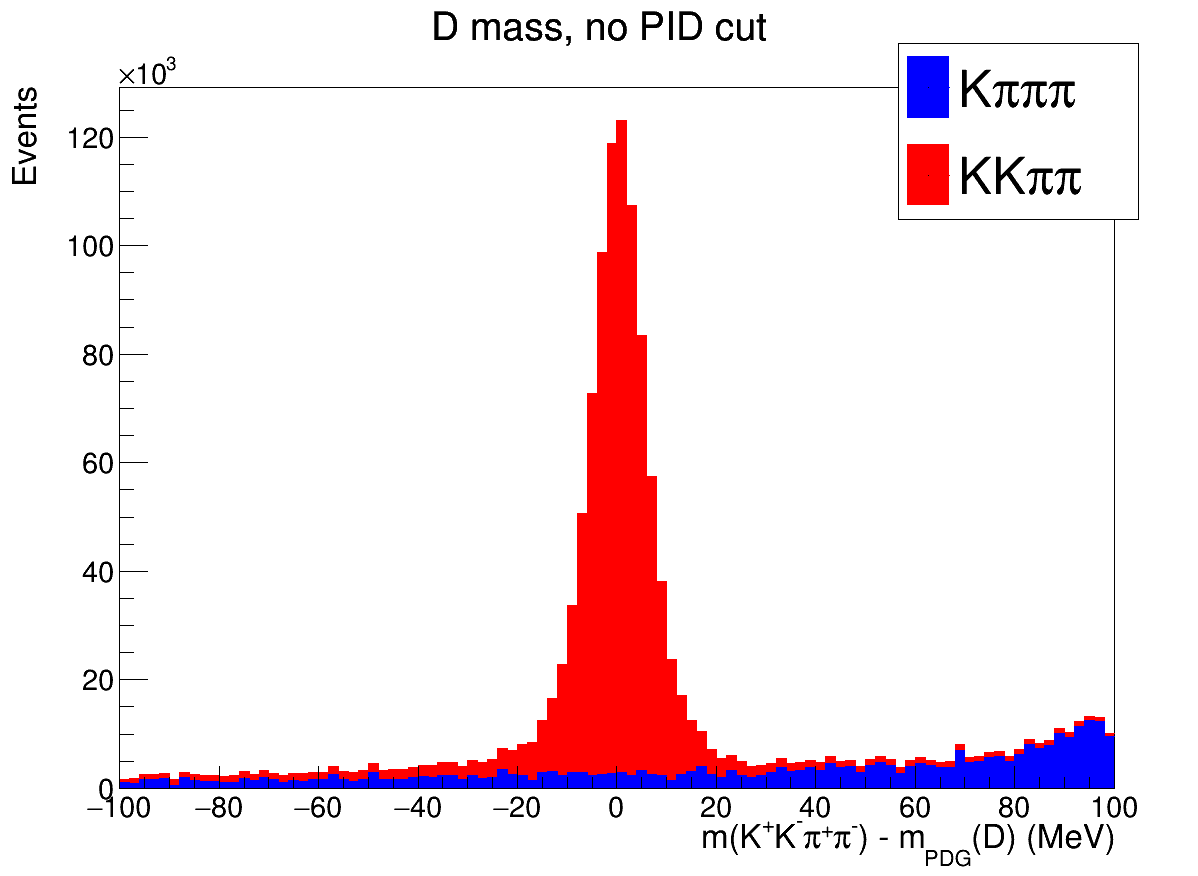
\includegraphics[width=1\textwidth]{Plots/B2DK_Dmass_Background.png}
    \caption{The $D$ invariant mass from $D\to K^+K^-\pi^+\pi^-$ and $D\to K^\pm\pi^\mp\pi^\pm\pi^\mp$ from simulated events.}
    \label{fig_Dmass_kpipipi}
  \end{subfigure}%
  \begin{subfigure}{0.5\textwidth}
    \centering
    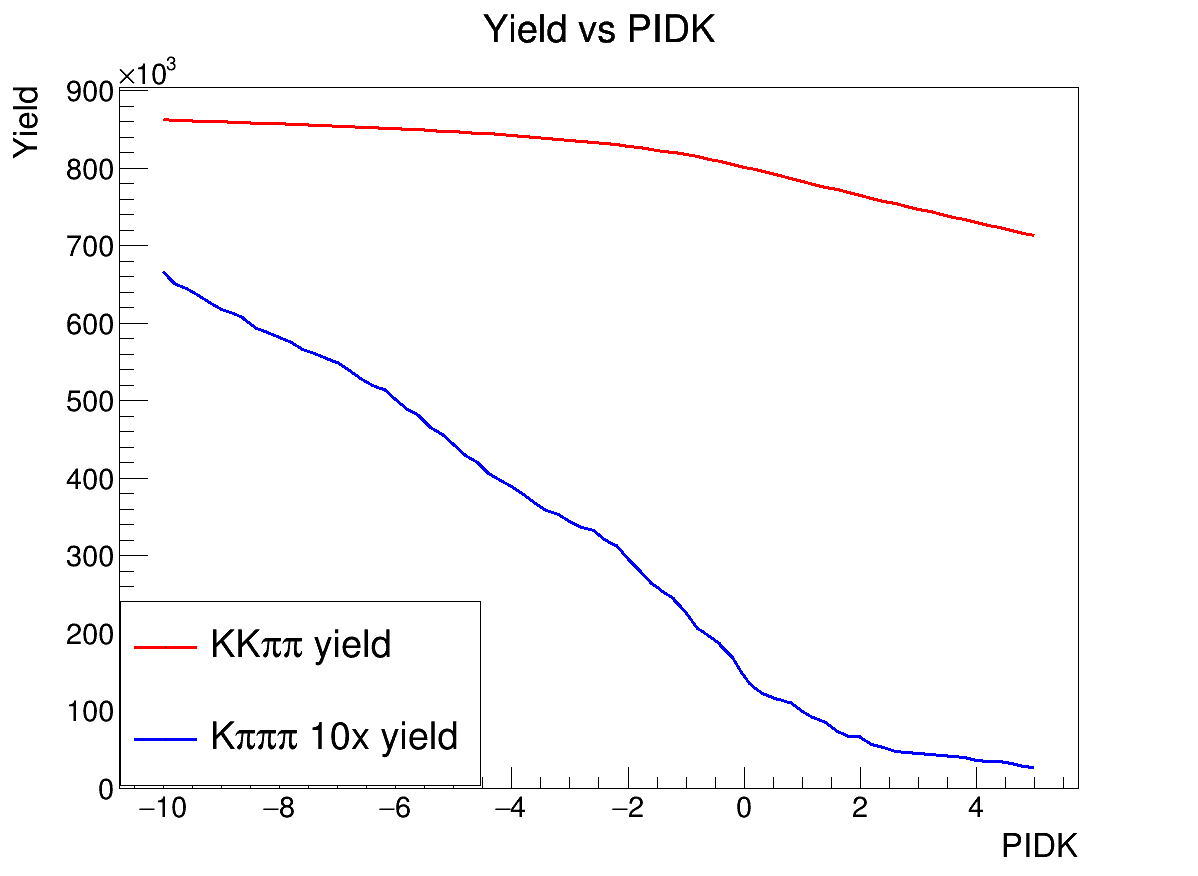
\includegraphics[width=1\textwidth]{Plots/YieldVSPIDK.png}
    \caption{The yield of $D\to K^+K^-\pi^+\pi^-$ and $D\to K^\pm\pi^\mp\pi^\pm\pi^\mp$ events as a function of $\text{PIDK}$.}
    \label{fig_yield_kpipipi}
  \end{subfigure}
  \caption{}
\end{figure}

A similar background from $D\to\pi^+\pi^-\pi^+\pi^-$ was found to be negligible because it requires two pions to be assigned the wrong hypothesis, which is very unlikely, and the $D$ invariant mass will be far outside the mass window.

\subsection{Charmless backgrounds}
\label{subsection_charmless}
\noindent Charmless backgrounds are $B^\pm$ candidates that decay directly into five charged tracks, without a charmed intermediate meson. These candidates will look like a signal in the $B^\pm$ invariant mass spectrum, but will form a continuous background in the $D$ invariant mass spectrum. A cut around the $D$ invariant mass will remove some of this background, but a large fraction will remain under the signal peak.

To estimate the amount of contamination, a separate selection was done without imposing a cut on the $\chi^2$ of the refitted $D$ daughters. This preserves the $D$ invariant mass sideband backgrounds, and a mass window in the lower sideband, $\SI{1770}{\mega\eV} < m(K^+K^-\pi^+\pi^-) < \SI{1820}{\mega\eV}$ was selected. The higher mass sideband was avoided due to contamination from $D\to K^\pm\pi^mp\pi^\pm\pi^\mp$. This mass window, which is of similar size to that of the signal mass window, contains real $B^\pm$, candidates, and the $B^\pm$ invariant mass is shown in Fig. \ref{fig_Bmass_charmless} for $B^\pm\to DK^\pm$ candidates.

\begin{figure}[H] 
  \centering
  \begin{subfigure}{0.5\textwidth}
    \centering
    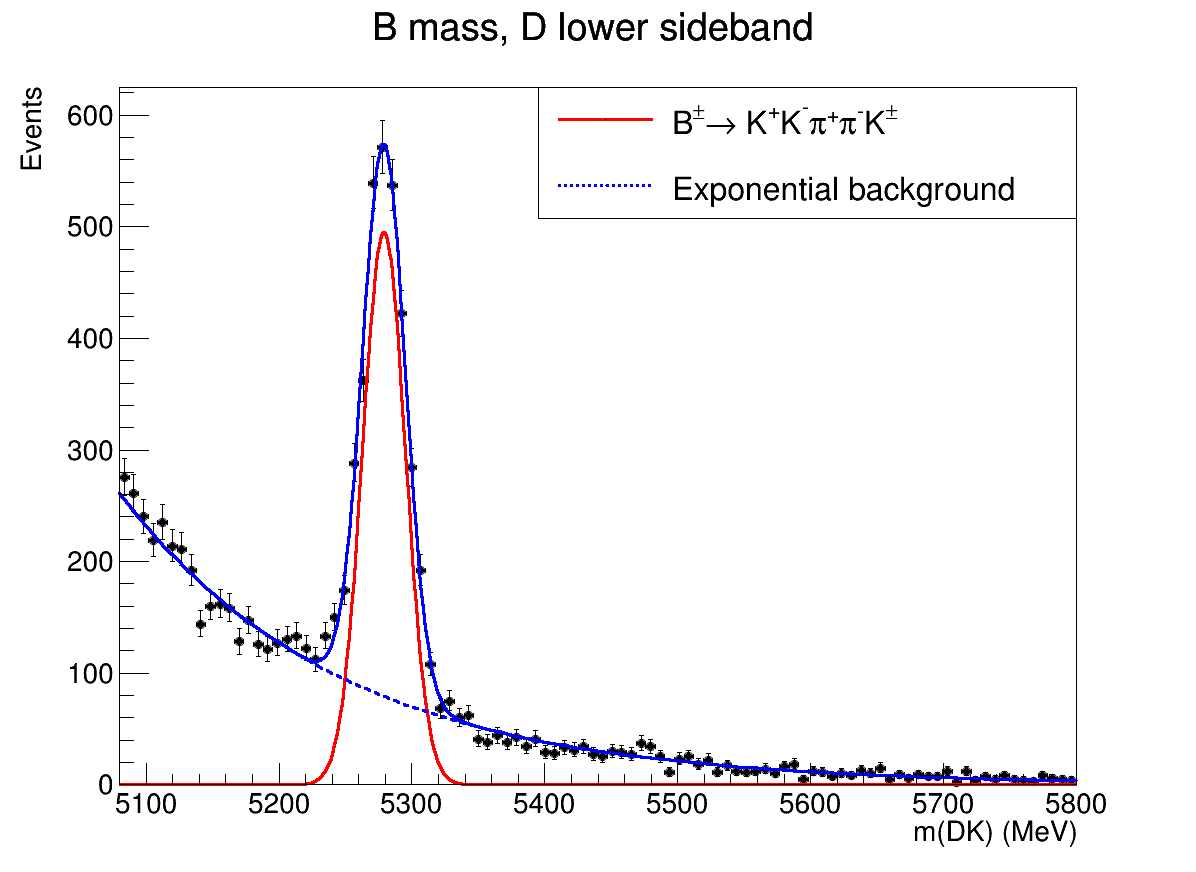
\includegraphics[width=1\textwidth]{Plots/B2DKLower_Charmless.png}
    \caption{The $B^\pm$ invariant mass in the $D$ invariant mass lower sideband.}
    \label{fig_Bmass_charmless}
  \end{subfigure}%
  \begin{subfigure}{0.5\textwidth}
    \centering
    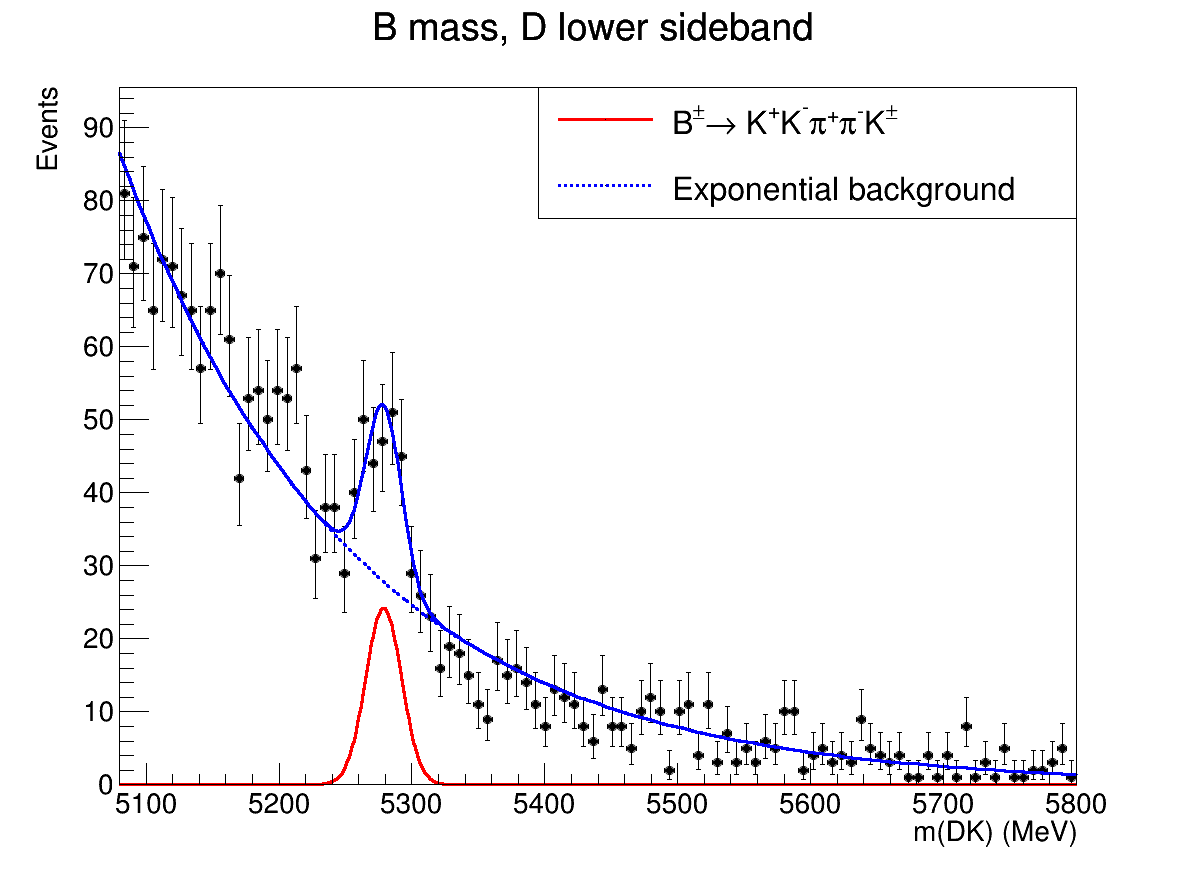
\includegraphics[width=1\textwidth]{Plots/B2DKLowerFDCut_Charmless.png}
    \caption{The $B^\pm$ invariant mass in the $D$ invariant mass lower sideband with a flight significance cut.}
    \label{fig_Bmass_charmless_fdcut}
  \end{subfigure}
  \caption{}
\end{figure}

A simple fit was performed on the spectrum in Fig. \ref{fig_Bmass_charmless}, with a Gaussian signal and an exponential background. The obtained yield was $\SI{2605(57)}{}$. The contamination from $B^\pm K^+K^-\pi^+\pi-K^\pm$ is therefore relatively large, compared to the expected signal yield of real $B^\pm\to (K^+K^-\pi+\pi^-)_DK^\pm$ candidates. However, no mass peak was found in the corresponding $B^\pm\to D\pi^\pm$ invariant mass spectrum, and therefore the charmless background $B^\pm\to K^+K^-\pi^+\pi^-\pi^\pm$ is negligible in the $B^\to (K^+K^-\pi^+\pi^-)\pi^\pm$ channel.

Since $D^0$ mesons travel a finite distance before decaying inside the VELO, a quantity called the flight significance, which is the flight distance divided by its error, may be defined. A preliminary cut was imposed such that only $B^\pm$ candidates with flight significance greater than $2.0$ are selected. This removes most of the charmless backgrounds, and the remaining background is shown in Fig. \ref{fig_Bmass_charmless_fdcut}. The yield after a flight significance cut is $\SI{110(19)}{}$.
%%%%%%%%%%%%%%%%%%%%%%%%%%%%%%%%%%%%%%%%%%%%%%%%%%%%%%%%%%%%%%%
\section{Fit to extract CP observables}
\subsection{Global fit and invariant mass spectra}
\label{section_global_fit}
\noindent A global maximum likelihood fit of all $B^\pm$ candidates was performed to determine the total yields and mass shape parameters in the $Dh^\pm$ invariant mass spectrum. The signal and background parameterization are the same as those in Ref. \ref{}, including which variables are floated in the fit and which are fixed. In addition, all fixed parameters are identical to the those in Ref. \ref{}, and only minor adjustments are needed for the final analysis.

The combinatorial background is parameterized as an exponentially falling background. The signal is parameterized as a sum of a Gaussian $f_\text{G}(m|m_B, \sigma)$ and a modified Gaussian that accounts for the radiate tail and wider resolution of signal events that are poorly reconstructed. The PDF has the form

\begin{equation}
  f_\text{MG}(m|m_B, \sigma, \alpha_L, \alpha_R, \beta)\propto
  \begin{cases}
    \exp\Big(\frac{-\Delta m^2(1 + \beta\Delta m^2)}{2\sigma^2 + \alpha_L\Delta m^2}\Big), \Delta m = m - m_B < 0 \\
    \exp\Big(\frac{-\Delta m^2(1 + \beta\Delta m^2)}{2\sigma^2 + \alpha_R\Delta m^2}\Big), \Delta m = m - m_B > 0 \\
  \end{cases}.
\end{equation}

To the left of the $B^\pm$ invariant mass peak are contributions from partially reconstructed backgrounds. These are mainly $B^\pm$ or $B^0$ decays to $D^*h^\pm$, and $D^*\to D\pi$ or $D^*\to D\gamma$, where the pion or photon are not reconstructed. The missing mass leads to peaking to the left of the signal. Furthermore, in the $B^\pm\to DK^\pm$, there is a component of $B^\pm\to D\pi^\pm$ candidates, where the $\pi^\pm$ daughter is wrongly assigned a kaon hypothesis. This is a small component to the right of the signal. Furthermore, this channel also has a component of $B_s\to DK^\pm\pi^\mp$ and the pion is not reconstructed, and a component of partially reconstructed background from $B^\pm$ and $B^0$ candidates where the $\pi^\pm$ daughter is mis-identified as a $K^\pm$. All partially reconstructed background components are fitted with PDF shapes described in Ref. \ref{}.

The final global fits for $B^\pm\to DK^\pm$ and $B^\pm\to D\pi^\pm$ are shown in Figs. \ref{fig_Bmass_B2DK} and \ref{fig_Bmass_B2Dpi}, respectively. The final yield of $B^\pm\to DK^\pm$ and $B^\pm\to D\pi^\pm$ candidates are $\SI{0(0)}{}$ and $\SI{0(0)}{}$, respectively.

\begin{figure}[H] 
  \centering
  \begin{subfigure}{0.5\textwidth}
    \centering
    \includegraphics[width=1\textwidth]{example-image-a}
    \caption{Global mass fit of $B^\pm\to DK^\pm$.}
    \label{fig_Bmass_B2DK}
  \end{subfigure}%
  \begin{subfigure}{0.5\textwidth}
    \centering
    \includegraphics[width=1\textwidth]{example-image-a}
    \caption{Global mass fit of $B^\pm\to D\pi^\pm$.}
    \label{fig_Bmass_B2Dpi}
  \end{subfigure}
  \caption{}
\end{figure}

\subsection{Binned CP fit and CP observables}
\noindent After the global fit described in Section \ref{section_global_fit}, $B^\pm$ candidates are split by charge and phase space bins, using the binning scheme described in Section \ref{section_binning_scheme}. A simultaneous maximum likelihood fit is performed for each charge and bin. All mass shape parameters are fixed from the global fit while the yield of signal, total partially reconstructed background and combinatorial background in each bin are floated.

The final fitted parameters are shown in Figs. \ref{fig_xpm_ypm}-\ref{fig_xxi_yxi}. Geometrically, the angle between the points $(x_+^{DK}, y_+^{DK})$ and $(x_-^{DK}, y_-^{DK})$ in Fig. \ref{fig_xpm_ypm} is $2\gamma$, and these six CP observables may be interpreted in terms of $\gamma$, $\delta_B^{DK}$, $r_B^{DK}$, $\delta^{D\pi}$ and $r_B^{D\pi}$. However, this step is only performed at the end to avoid any human bias in the final result.

\begin{figure}[H] 
  \centering
  \begin{subfigure}{0.5\textwidth}
    \centering
    \includegraphics[width=1\textwidth]{example-image-a}
    \caption{Confidence levels at $68.2\%$ and $95.5\%$ of $(x_+^{DK}, y_+^{DK})$ and $(x_-^{DK}, y_-^{DK})$.}
    \label{fig_xpm_ypm}
  \end{subfigure}%
  \begin{subfigure}{0.5\textwidth}
    \centering
    \includegraphics[width=1\textwidth]{example-image-a}
  \caption{Confidence levels at $68.2\%$ and $95.5\%$ of $(x_\xi^{D\pi}, y_\xi^{D\pi})$.}
    \label{fig_xxi_yxi}
  \end{subfigure}
\end{figure}

\subsection{Validation of fit procedure with toy studies}
\noindent To ensure that the fit procedures are robust, for both the global and CP fit $1000$ toy datasets are generated with the fitted parameters. Each toy datasets is then run through the same fitting procecure and the pull distibutions of each floated variable is studied closely. It was found that no CP observables were biased or had any understimated errors. Two nuisance parameters in the global fit had slightly underestimated errors which are easily corrected for.

%%%%%%%%%%%%%%%%%%%%%%%%%%%%%%%%%%%%%%%%%%%%%%%%%%%%%%%%%%%%%%%
\section{External strong phase input from BESIII}
\noindent Analysis of the BESIII data consists of $e^+e^-$ collisions at the $\psi(3770)$ resonance. In addition, there exists inclusive simulated samples of each category of events. The relevant category for this analysis is $D^0\bar{D^0}$ events, which has $21.8$ times more simulated events relative to data. Simulations of exclusive processes are generated when needed.

The most important aspects of this analysis is reconstructing single and double tagged event yields. Peaking backgrounds must be accounted for using the inclusive simulation samples. Finally, the yields are inputted into a maximum likelihood fit using Eqs. \eqref{eq_Mi}-\eqref{eq_Mij} to obtain $c_i$ and $s_i$.

Since an $e^+e^-$ collider is a very clean environment, charged and neutral particles mostly follow the same reconstruction strategy, described in Ref. \ref{}. Since the beams are symmetric, each $D$ meson must have energy $E_\text{beam}$. When the daughters of a $D$ meson is reconstructed, the energy difference $\Delta E$ and beam-constrained mass $M_\text{BC}$ may be defined as

\begin{equation*}
  \Delta E = \sum_i E_i - E_\text{beam}, \quad M_\text{BC} = \sqrt{E_\text{beam}^2 - \abs{\sum_i\vb{p}_i}^2}.
\end{equation*}

For a perfectly reconstructed $D$ meson, $\Delta E = 0$. However, due to detector resolution it is a peak of finite width. In addition, for tag modes with photon showers, the $\Delta E$ distribution has a left tail due to energy leakage through the calorimeter. The beam-constrained mass can be interpreted as the $D$ invariant mass, but using the well measured beam energy to improve the resolution.

\subsection{\texorpdfstring{$K_S^0$}{KS0} veto}
\noindent The main peaking background in this analysis is $D\to K_S^0K^+K^-$, where $K_S^0\to\pi^+\pi^-$. It has the same experimental signature as $D\to K^+K^-\pi^+\pi^-$ and therefore forms a signal peak in the $M_\text{BC}$ distribution. Most of this background is removed with a flight significance cut at $2.0$. The remaining background is from $K_S^0K^+K^-$ candidates where the $K_S^0$ decays close to the primary vertex, making it impossible to distinguish from $D\to K^+K^-\pi^+\pi^-$. This remaining background is therefore removed by imposing a veto on the $\pi^+\pi^-$ invariant mass. A sample of simulated $D\to K_S^0K^+K^-$ events was generated, but reconstructed as $D\to K^+K^-\pi^+\pi^-$ and the $\pi^+\pi^-$ invariant mass was studied. It was found that an asymmetric veto of $\SI{477}{\mega\eV} < m_{K_S^0} < \SI{507}{\mega\eV}$ was more efficient in removing this peaking background. After the veto, a negligible amount of the peaking background remained.

\subsection{Single tag yield}
\noindent The single tag yield is obtained by reconstructing events where one of the $D$ mesons decay into a tag mode, while the other $D$ meson is not reconstructed. A mode-dependent cut on $\Delta E$ is chosen by fitting a double Gaussian for the signal peak and a second order polynomial for the background in the $\Delta E$ distribution. A cut around $\pm 3\sigma$ is performed to remove combinatorial background. For modes with photon showers, the left cut is extended to $-4\sigma$.

The single tag yield is then obtained by fitting the $M_\text{BC}$ distribution. The continuous combinatorial background is modelled with an Argus shape. The signal shape is taken from a simulated sample of the signal, convolved with a Gaussian to account for detector resolution. Peaking backgrounds, if present, are accounted for with Gaussian shapes, with shape and yield fixed from the inclusive MC samples. An example of such a fit is shown in Fig. \ref{fig_styield}.

\subsection{Double tag yield}
\noindent The double tagged yield is obtained by reconstructing both $D$ mesons. The same cuts on $\Delta E$ used for single tagged events are applied, and the beam constrained mass for both $D$ mesons are plotted in a $2$D scatter plot, shown in Fig. \ref{fig_dtyield}. Since the yields are expected to be too low for a maximum likelihood fit, a sideband subtraction technique is employed instead.

\begin{figure}[H] 
  \centering
  \begin{subfigure}{0.5\textwidth}
    \centering
    \includegraphics[width=1\textwidth]{example-image-a}
    \caption{Fit of single tagged $M_\text{BC}$ distribution to obtain single tag yields.}
    \label{fig_styield}
  \end{subfigure}%
  \begin{subfigure}{0.5\textwidth}
    \centering
    \includegraphics[width=1\textwidth]{example-image-a}
  \caption{Background subtraction technique of double tagged $M_\text{BC}$ distributions to obtain double tag yields}
    \label{fig_dtyield}
  \end{subfigure}
\end{figure}

The $M_\text{BC}$ region in Fig. \ref{fig_dtyield} is split into $5$ regions. Region $S$ is the signal region, while $A$ and $B$ are events where one of the $D$ mesons are correctly reconstructed. Region $C$ are real events but daughter tracks between the $D$ mesons have been swapped. Finally, region $D$ contains purely combinatorial background. The total background is estimated using

\begin{equation*}
  B = P + \frac{a_S}{a_D}Y_D + \sum_{i = A, B, C}\frac{a_S}{a_i}\Big(Y_i - \frac{a_i}{A_D}Y_D\Big),
\end{equation*}
where $P$ is the peaking background found from inclusive MC, $Y_i$ is the yield in region $i$ and $a_i$ is the corresponding area of the region.

Since the current dataset is insufficient for extracting $c_i$ and $s_i$, it is more instructive to compare the double tag yields with the prediction from the LHCb amplitude model. In Fig. \ref{fig_flavour_yield}, $D\to K^+K^-\pi^+\pi^-$ the yield of events tagged with the flavour tag $D\to K^\pm\pi^\mp$ are shown (data points), with the amplitude model prediction (solid line). The events have been binned using a $2\times 4$ binning scheme as described in Section \ref{section_binning_scheme}. In Fig. \ref{fig_cp_yield}, an equivalent plot for the $D\to K^+K^-\pi^+\pi^-$ events, tagged with a CP even tag mode $D\to K^+K^-$ and a CP odd tag mode $K_S^0\pi^0$, without binning. Overall, the data looks consistent with the model prediction.

\begin{figure}[H] 
  \centering
  \begin{subfigure}{0.5\textwidth}
    \centering
    \includegraphics[width=1\textwidth]{example-image-a}
    \caption{Binned double tag yield of $K^+K^-\pi^+\pi^-$ versus $K^\pm\pi^\mp$ events.}
    \label{fig_flavour_yield}
  \end{subfigure}%
  \begin{subfigure}{0.5\textwidth}
    \centering
    \includegraphics[width=1\textwidth]{example-image-a}
  \caption{Inclusive double tag yield of $K^+K^-\pi^+\pi^-$ versus $K^+K^-$ and $K_S^0\pi^0$ events.}
    \label{fig_cp_yield}
  \end{subfigure}
\end{figure}

%%%%%%%%%%%%%%%%%%%%%%%%%%%%%%%%%%%%%%%%%%%%%%%%%%%%%%%%%%%%%%%
\section{Discussion of future work}
\noindent Discuss the future plans with Guy first!


%%%%%%%%%%%%%%%%%%%%%%%%%%%%%%%%%%%%%%%%%%%%%%%%%%%%%%%%%%%%%%%                                                                          
\bibliography{references}
\bibliographystyle{unsrt}

%%%%%%%%%%%%%%%%%%%%%%%%%%%%%%%%%%%%%%%%%%%%%%%%%%%%%%%%%%%%%%%
\newpage
\section{DPhil thesis plan}
\noindent Discuss DPhil thesis plan with Guy first!

\end{document}